\section{Імплементація методу лапароскопічної резекції печінки в практику}

Згідно рекомендацій третьої погоджувальної конференції в Саузхемптоні лапароскопічні резекції печінки рекомендовані до впровадження в центрах, що мають достатній досвід як резекційної печінкової так і лапароскопічної хірургії \cite{AbuHilal2017a}. Імплементація \acrshort{llr} повинна бути етапною, з поступовим збільшенням складності втручаннь. 

\subsection{Оцінка складності лапароскопічних резекцій печінки}
Для ефективного відбору пацієнтів на етапі імплементації необхідна об'єк\-тивна оцінка складності втручання. З цією метою запропоновано декілька систем, які прогнозують ризики розвитку ускладненнь після \acrshort{llr} \cite{Kawaguchi2018, Hasegawa2017a}. Найбільш широко вживана з цих систем, яка пройшла зовнішню валідацію, це IWATE-score (Таб.\ref{table:iwate}), названа так на честь префектури в Японії, де була розроблена \cite{Ban2014}. Система враховує локалізацію, розмір пухлини, близькість процесу до магістральних внутрішньопечінкових структур, необхідний об'єм резекції та  ступінь печінкової недостатності за Чайлдом. На основі оцінки цих факторів резекція оцінюється в балах складності від 1 до 10 (Таб.\ref{table:iwate-score}). Наявність 1-3 балів свідчить про низьку складність, 4-6 - середню складність, 7-10 - високу складність. 

Складність LLR
\begin{table}
\begin{tabular}{ |p{0.15\linewidth} |p{0.05\linewidth} |p{0.05\linewidth}|p{0.05\linewidth}|p{0.05\linewidth}|p{0.05\linewidth}|p{0.05\linewidth}|p{0.05\linewidth}|p{0.05\linewidth}|p{0.05\linewidth}|p{0.05\linewidth}|p{0.05\linewidth}| }
\hline
\multicolumn{11}{|c|}{Складність \acrshort{llr}} \\
\hline
Бали & 1 & 2 & 3 & 4 & 5 & 6 & 7 & 8 & 9 & 10 \\
\hline
Складність   & \multicolumn{3}{p{0.15\linewidth}|}{Низька} & \multicolumn{3}{p{0.15\linewidth}|}{Середня} & \multicolumn{4}{p{0.20\linewidth}|}{Висока} \\
\hline
Визначення   & \multicolumn{3}{p{0.20\linewidth}|}{Для хірургів що починають \acrshort{llr} з досвідом до 10 операцій} & \multicolumn{3}{p{0.20\linewidth}|}{Для хірургів, що успішно виконють \acrshort{llr} низької складності з досвідом 10-50 операцій } & \multicolumn{4}{p{0.25\linewidth}|}{Для хірургів, що успішно виконють \acrshort{llr} середньої складності з досвідом більше 50 операцій } \\
\hline
\end{tabular}

\caption{\label{table:iwate}Індекси IWATE для оцінки складності \acrshort{llr} }
\end{table}





Бали складності
\begin{table}
\begin{tabular}[t]{ |p{0.5\textwidth}| p{0.3\textwidth}|  }
\hline
   \textbf{Локалізація ураження} & \textbf{Розмір ураження} \\

\multirow{6}{*}{
  % \rule{0pt}{100pt}   % Висота строки 
   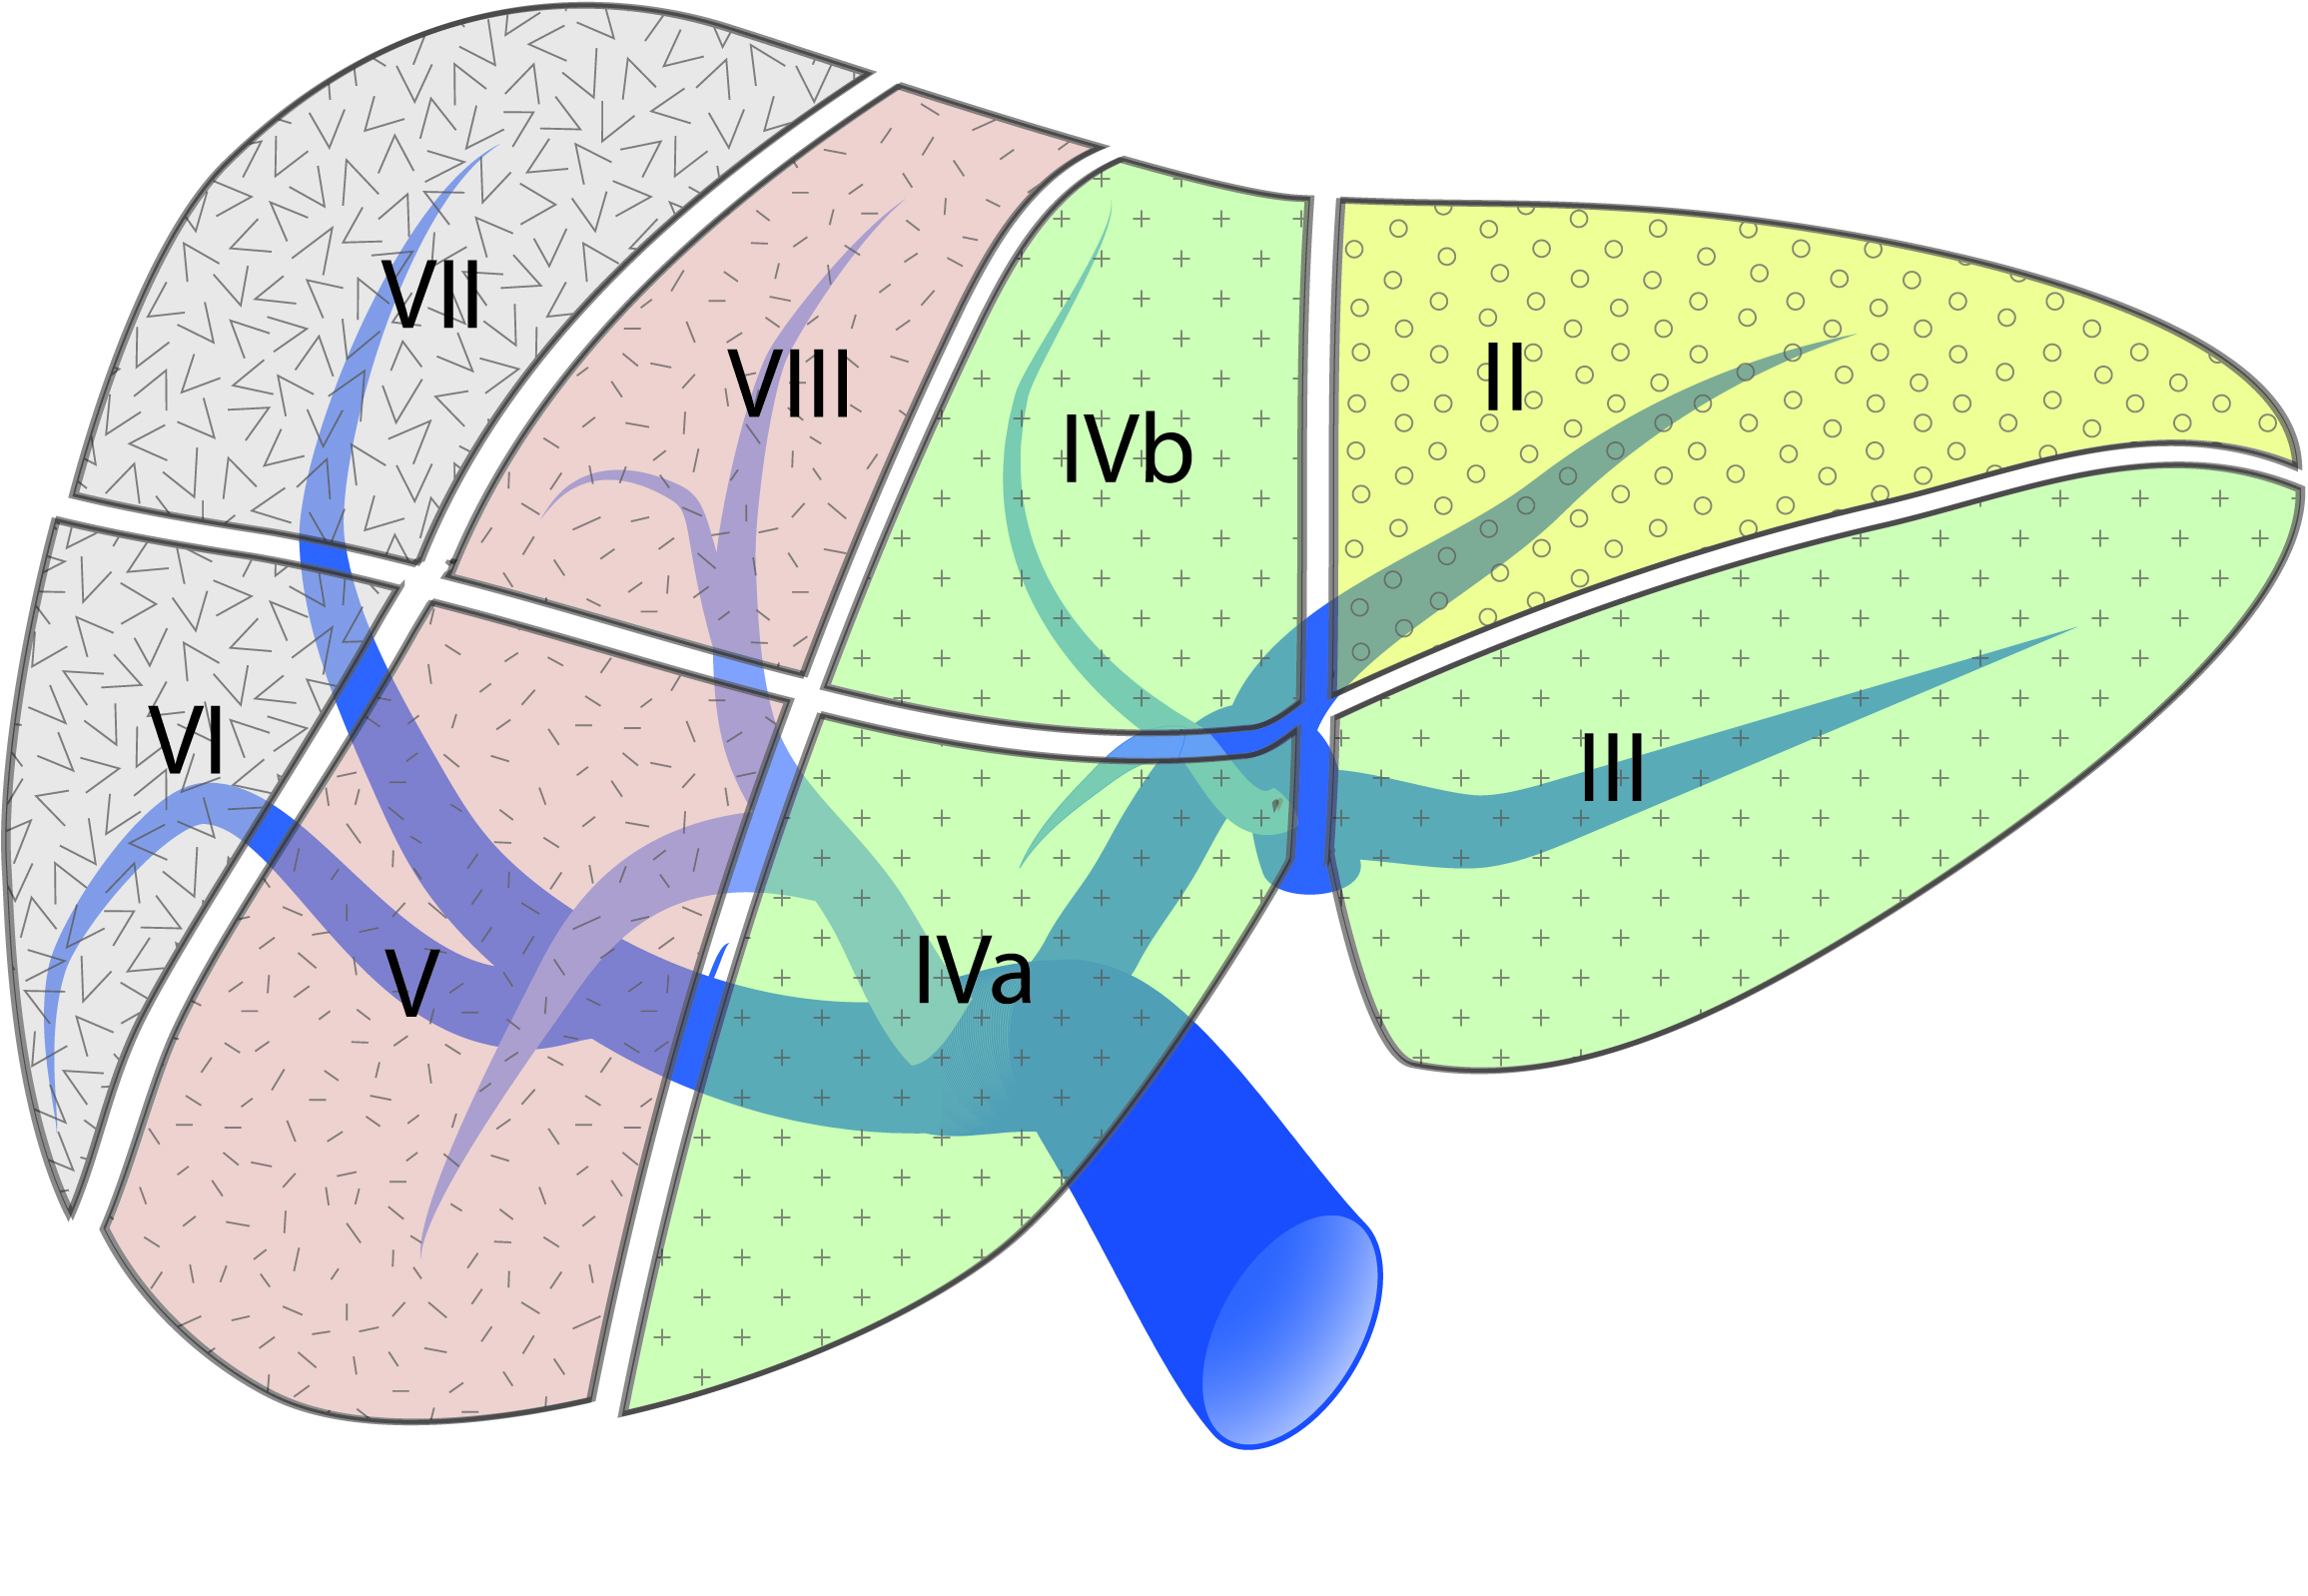
\includegraphics[width=0.3\textwidth]{Illustrations/Chapter_01/Couinaud.jpg} 
    \begin{tabular}{c|c} 
       Sg & Бали \\ %[0.5ex] 
       \hline\hline
       2 & 2 \\ 
       3 & 1 \\ 
       4 & 3 \\ 
       5 & 3 \\ 
       6 & 2 \\ 
       7 & 5 \\ 
       8 & 5 \\ 
    \end{tabular}
  }
& \begin{centre}
   \begin{tabular}[t]{c c} 
     & Бали \\
     <3 см & 0 \\ 
    \geq 3 см & 1 \\ 
    
   \end{tabular}
 \end{centre} \\
& \textbf{Близькість до судин} \\ 
& \begin{centre}
   \begin{tabular}{c c} 
%      & Бали \\
     Відсутня & 0 \\ 
     Наявна & 1 \\ 
   \end{tabular}
 \end{centre} \\
 & \\
 & \\
 & \\
\hline  
\textbf{Об'єм резекції} & \textbf{Функція печінки} \\   %

  \begin{centre}
   \begin{tabular}{c c} 
     & Бали \\
     Парціальна резекція & 0 \\ 
     \acrshort{llls} & 2 \\ 
     Сегментектомія & 3 \\ 
     Не менше секцієеткомії & 4 \\
   \end{tabular}
 \end{centre}  
& \begin{centre}
   \begin{tabular}{c c} 
     & Бали \\
     Child-Pugh A & 0 \\ 
     Child-Pugh B & 1 \\ 
   \end{tabular}
 \end{centre} \\
\hline                  
\end{tabular}
\caption{\label{table:iwate-score}Шкала IWATE складності \acrshort{llr} }
\end{table}

\subsection{Етапи впровадження лапароскопічних резекцій печінки}
Процес імплементації \acrshort{llr} повинен бути системним, а в процес навчання повинна бути залучена вся хірургічна бригада (оператори, асистенти, анестезіологи, операційні сестри). Крива навчання для малих резекцій печінки складає 60 випадків, а для великих цей показник складає 55 випадків. Проходження хірургічною бригадоб кривої навчання малих резекцій може знизити цей показник для великих резекцій. Враховуючи це, запровадження програми \acrshort{llr} має сенс лише в госпіталях, в яких виконується більше 50 відкритих резекцій на рік \cite{Vigano2009, Hasegawa2017, Marcel2016}. 
Основні етапи, що має пройти клініка при впровадженні програми наступні:

\begin{enumerate}
    
   \item \textbf{Теоретична підготовка та матеріально-технічне забезпечення.} На цьому етапі оцінюють потенційну потребу клініки в \acrshort{llr} та відповідно неї формують одну чи декілька хірургічних бригад. Після проходження персоналом стажування в клініках з великим об'ємом \acrshort{llr} та набуттям початкового досвіду формується перелік необхідного обладнання та інструментів. 
    
   \item \textbf{Проходження кривої навчання малих \acrshort{llr}.} Для проходження цього етапу відбирають пацієнтів із ураженнями антеролатеральних сегментів невеликого розміру, на значному віддаленні від магістральних структур. Для перших 10 втручаннь необхідні випадки із рівнем складності 1-3 балів за шкалою IWATE (як правило це крайові парціальні резекції вогнищ < 3 см у пацієнтів без циррозу). Починаючи із 11 випадку рекомендовано збільшувати складність до 4-6 балів за шкалою IWATE за ракунок анатомічних сегментектомій антеролатеральних сегментів та лівої латеральної секцієектомії. Мета цього етапу - відпрацювання базових елементів техніки \acrshort{llr} таких, як прийом Прінгла, мобілізація лівої та правої долей печінки, транссекція паренхіми, гемостаз, диссекція та лігування лівої печінкової вени.
    
   \item \textbf{Проходження кривої навчання великих \acrshort{llr}.} Після успішного проходження кривої навчання малих резекції (~ 60 випадків) переходять до виконання великих резекцій печінки (3 або більше суміжних сегменти), та підвищують поріг складності операцій до 7-10 балів за шкалою IWATE. Для цього підбирають випадки із утвореннями більшого розміру, включаючи локалізацію у правій долі та важкодоступних сегментах 7 та 8. На цьому етапі відпрацьовують такі складні елементи техніки \acrshort{llr} як  ізольована або гліссон-орієнтована диссекція правих портальних структур, диссекція запечінкового відділу \acrshort{ivc}, диссекція та лігування \acrshort{rhv}, транссекція паренхіми при великих новоутвореннях. Починають етап із виконання правобічних та лівобічних гемігепатектомій, потім переходять до секцієектомій та мезогепатектомій та при їх успішному опануванні виконують анатомічні резекції Sg 7 та 8. 
    
   \item \textbf{Введення \acrshort{llr} в стандарти надання допомоги клінікою.} Після проходження хірургічною бригадою кривої навчання \acrshort{llr} може бути закріплена в протоколі надання допомоги пацієнтам із вогнищевою патологією печінки як один з можливих методів. Для пацієнтів із ураженням антеролатеральних сегментів \acrshort{llr} є стандартом практики. Після імплементації \acrshort{llr} в сучасному відділенні гепатобіліарної хірургії high-volume центру їх доля як правило сягає 30-80\% від загального числа резекцій печінки. 

\end{enumerate}